\documentclass[twoside,10pt]{article}
\usepackage{/Users/bradenhoagland/latex/styles/toggles}
%\toggletrue{sectionbreaks}
%\toggletrue{sectionheaders}
%\toggletrue{separateTitlePage}
\newcommand{\docTitle}{Natural Gradient Methods for Optimization and Applications to Reinforcement Learning}
\usepackage{/Users/bradenhoagland/latex/styles/common}
\importStyles{formal}{rainbow}{plain}


\usepackage[superscript]{cite}
\usepackage{algorithm, algpseudocode, graphicx}
\usepackage[margin=1in,font=small]{caption}
\usepackage{subfig}


\newcommand{\subheader}[1]{\bigskip\begin{center}\textbf{#1}\end{center}}
\newcommand{\subsubheader}[1]{\bigskip\begin{center}\textit{#1}\end{center}}

\begin{document}

% =====
% TITLE
% =====
\formalTitle{\docTitle}{Braden Hoagland}{Math 361S: Numerical Analysis}
\formalHeader{Braden Hoagland}{The Natural Gradient and Reinforcement Learning}


% ========
% ABSTRACT
% ========
\vspace{10mm}
%\subheader{Abstract}
\begin{abstract}
Although widely used as a simple method for optimization, traditional gradient descent is not optimal on general metric spaces. An extension of this method, natural gradient descent, empirically exhibits better convergence rates by modifying the gradient of a function to point in the steepest descent direction of the metric space of the particular problem. This generalization is of particular use in the field of reinforcement learning, where the modification of the gradient reduces to a left-multiplication by the inverse of the Fisher information matrix. The inclusion of this matrix in policy gradient methods empirically speeds up policy improvement, and an efficient calculation of the matrix-gradient product using the conjugate gradient can be employed to scale this method to larger problems.
\end{abstract}


% ============
% INTRODUCTION
% ============
\subheader{Introduction}
Gradient descent is a widely-used used method for minimizing nonlinear equations, and its stochastic variant is a common way of fitting models to large amounts of data. Although it is follows the direction of steepest descent in Euclidean spaces, it does not do so on general manifolds.\cite{amari} This issue mainly arises due to differing notions of the gradient of a function on different spaces, but can be addressed by introducing a regularizer. This takes the form of a matrix that modifies the Euclidiean gradient to be correct in more general metric spaces, and is referred to as the ``natural gradient".

In this paper, we will motivate the natural gradient using the gradient descent framework, then highlight its properties when applied specifically to gradient descent on probability spaces. We will then show its applications to the field of reinforcement learning, in which it has been used to create state-of-the-art algorithms for continuous control tasks.\cite{peters-schaal, trpo}

% ==================================
% GRADIENT DESCENT AND TRUST REGIONS
% ==================================
\subheader{Gradient Descent and Trust Regions}
In gradient descent, one of the simplest methods of optimization, a differentiable function $f(x)$ is optimized iteratively by following the direction of steepest descent, i.e., the gradient. An iteration for this method can be written
\begin{gather*}
    x_{t+1} = x_t - \alpha_t \nabla f(x_t),
\end{gather*}
where $\alpha$ is a step size chosen small enough to keep the local gradient information accurate. An exact line search for $\alpha_t$ makes each step more efficient, but is only feasible when computing the minimum of $f(x)$ along a given search direction is cheap. This occurs when the form of $f(x)$ is known and well understood, such as $f(x)$ being quadratic. For arbitrary functions, a backtracking line search may be used instead. An optimistic $\alpha$ is chosen and then repeatedly decreased until a decrease condition on $f(x_t + \alpha_t \nabla f(x_t))$ is met. A simpler method is to just use a fixed step size, although the performance of this is strictly worse than that of the line search methods.

Gradient descent can also be viewed as a trust region method.\cite{tr} Trust region methods construct a model of $f(x)$ that has bounded error over some small region around the current iterate. This model is constructed in such a way that it can be easily optimized at each step. The optimization of $f(x)$ reduces to the optimization of many smaller sub-problems, namely the optimization of many locally-accurate models of $f(x)$.

In the particular case of gradient descent, the model is linear and a constraint is placed on the distance between iterates $x_t$ and $x_{t+1}$.
\begin{gather*}
    x_{t+1} = \arg\min_x f(x_t) + \nabla f(x_t)^T (x-x_t) \\
    \text{s.t. } \Vert x - x_t \Vert = \delta_t,
\end{gather*}
where $\delta_t \geq 0$ is some constant that depends on the step size $\alpha_t$. In the case of a fixed step size $\alpha$, we have $\delta_t = \delta \; \forall t$. The constraint can be equivalently written
\begin{gather*}
    \frac{1}{2} \Vert x - x_t \Vert^2 = \frac{\delta^2}{2} =: \varepsilon,
\end{gather*}
which will allow for simplified computation later on. Gradient descent is formulated using the Euclidean norm, but this can be unsatisfying. Such a choice imposes a Euclidean geometry on $f(x)$, which leads to a geometric mismatch when a non-Euclidean function is being optimized.

A simple example is the optimization of probability distributions parameterized by $x_t$. Suppose $x_t = (\mu_t, \sigma_t)$, where $\mu_t$ and $\sigma_t$ are, respectively, the mean and standard deviation of a univariate Gaussian distribution. In this case, we can generate distributions which are significantly different in a qualitative sense but have the same Euclidean distance from each other in terms of $x_t$.

\begin{figure}[H]
    \centering
    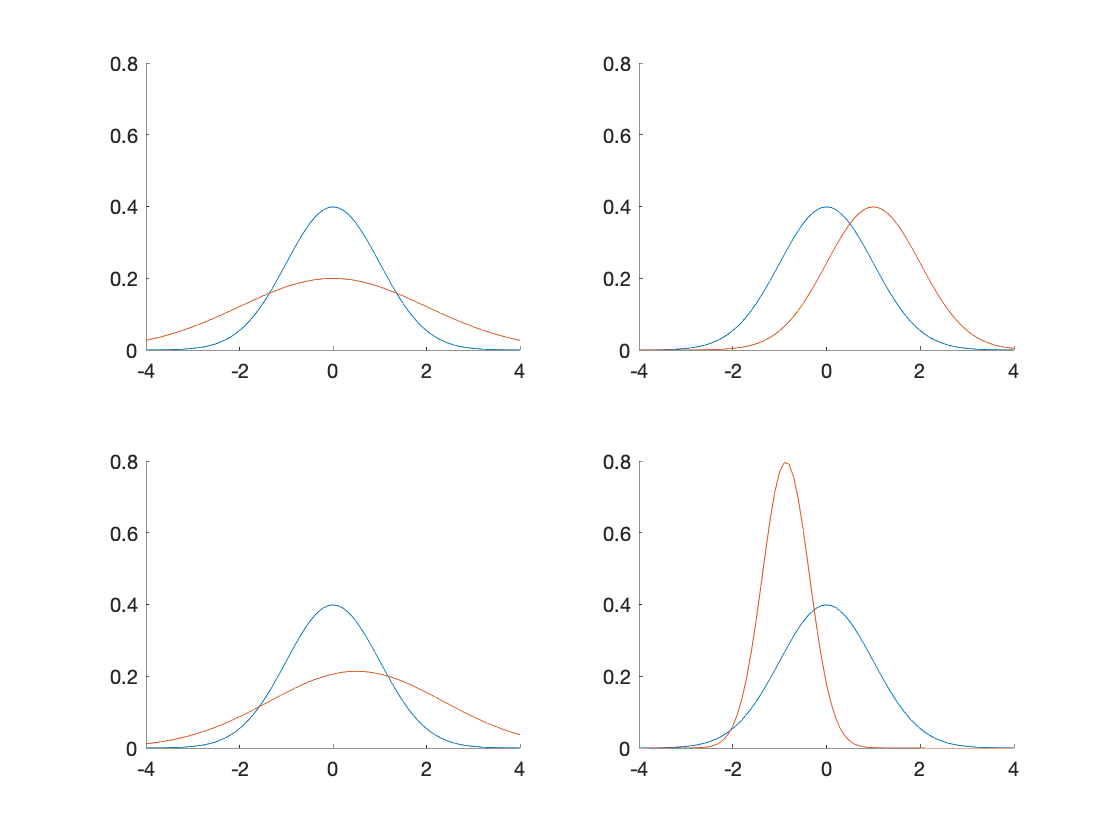
\includegraphics[width=9cm]{img/gaussians.png}
    \caption{The parameters of the orange distributions all have the same Euclidean distance from the parameters of the blue distribution, yet each orange distribution is considerably qualitatively different.}
\end{figure}

In fact, for Riemannian manifolds in general, the gradient isn't the steepest descent direction.\cite{amari} The direction of steepest descent for a function $f$ on a manifold is defined as follows: it is the vector $dx$ that minimizes $f(x+dx)$ under the constraint that $\vert dw \vert^2$ is a sufficiently small constant. In Euclidean space, $\vert dw \vert^2 = \sum_i \vert dx_i \vert^2$, so gradient descent uses the correct notion of distance. On a Riemannian manifold, however, this form is a more general quadratic $\vert dw \vert^2 = \sum_{i,j} g_{ij}(x) \, dx_i \, dx_j = x^T G x$. The elements $g_{ij}$ make up what's called the metric tensor $G$ for the coordinate system based on $x$.\cite{amari}

We can describe a point on a general manifold by transforming a point from the base coordinates using the metric tensor $G$. Intuitively, this matrix weights certain dimensions in our base coordinate system more than others when describing distance in the corresponding metric space.

% =================================
% NATURAL GRADIENT ON METRIC SPACES
% =================================
\subheader{The Natural Gradient on Metric Spaces}

To incorporate this notion of distance into the gradient descent formulation, we modify the Euclidean norm to be weighted by $G$. This gives us a gradient descent scheme with a slightly modified trust region constraint
\begin{gather*}
    x_{t+1} = \arg\min_x f(x_t) + \nabla f(x_t)^T (x-x_t) \\
    \text{s.t. } \frac{1}{2} \Vert x - x_t \Vert^2_{\color{blue}G} = \varepsilon,
\end{gather*}
where the norm now takes on the form $\Vert x \Vert^2_G = x^T G x$. This particular constrained optimization problem can be solved straightforwardly using the method of Lagrange multipliers. The general strategy we will follow is to first determine the optimal update direction, then find the maximum step size such that the trust region constraint is not violated.

We begin by forming the Lagrangian, which for this problem is
\begin{gather*}
    \mathcal{L}(x, \lambda) = f(x_t) + \nabla f(x_t)^T (x-x_t) - \lambda \Big( \frac{1}{2} \Vert x - x_t \Vert_G^2 - \varepsilon \Big).
\end{gather*}
To find the optimal search direction, we can find the optimal $d = x - x_t$.
\begin{align*}
    \frac{\partial \mathcal{L}}{\partial d} &= 0 \\
	\nabla f(x_t) - \lambda G d &= 0 \\
	d &= \frac{1}{\lambda} G^{-1} \nabla f(x_t).
\end{align*}
Thus the optimal update is in the direction of $G^{-1} \nabla f(x_t)$. This means we can form an update rule based on gradient descent, but using this modified gradient as the descent direction.
\begin{gather*}
    x_{t+1} = x_t - \beta G^{-1} \nabla f(x_t),
\end{gather*}
where $\beta$ is a currently unknown step size that takes the place of the $\frac{1}{\lambda}$ term. The term $G^{-1} \nabla f(x_t)$ is not only a descent direction, it is in fact the direction of steepest descent on a general Riemannian manifold.\cite{amari}

This update rule is still incomplete, however, since the optimal step size $\beta$ is unknown. Fortunately, we can solve for $\beta$ analytically using the update rule and the trust region constraint.
\begin{align*}
    \frac{1}{2} \Vert x_{t+1} - x_t \Vert_G^2 &= \varepsilon \\
    \frac{1}{2} \Vert - \beta G^{-1} \nabla f(x_t) \Vert_G^2 &= \varepsilon \\
    \frac{1}{2} \beta^2 \Vert G^{-1} \nabla f(x_t) \Vert_G^2 &= \varepsilon \\
    \beta &= \sqrt{\frac{2 \varepsilon}{\Vert G^{-1} \nabla f(x_t) \Vert_G^2}}.
    \intertext{Since $\varepsilon = \frac{1}{2} \delta^2$, this can be simplified to}
    \beta &= \frac{\delta}{\Vert G^{-1} \nabla f(x_t) \Vert_G}.
\end{align*}
Substituting this into our update rule, we get
\begin{align*}
    x_{t+1} &= x_t - \beta G^{-1} \nabla f(x_t) \\
    x_{t+1} &= x_t - \delta \frac{G^{-1} \nabla f(x_t)}{\Vert G^{-1} \nabla f(x_t) \Vert_G}.
\end{align*}
This final expression is easily connected with standard gradient descent. Letting $G=I$ (which is the case if we are optimizing a function in Euclidean space), we recover the standard gradient descent formulation with a normalized gradient.

We refer to $G^{-1} \nabla$ as the ``natural gradient". We also make two other notation decisions. First, to preserve the use of only one modifiable constant, we use the variant of the step size that is based on $\varepsilon$ (this is mainly based on convention). Second, to emphasize the computation required to compute the squared $G$-weighted norm, we express it in its $x^T G x$ form instead of the $\Vert \cdot \Vert^2_G$ form.

With these notation decisions in place, we can formally summarize the natural gradient method in Algorithm~\ref{alg:NGD}.

% ~~~~~~~~~~~~~~~~~~~~~~~~~~~~~~~
% ALGORITHM: NGD ON METRIC SPACES
% ~~~~~~~~~~~~~~~~~~~~~~~~~~~~~~~
{\centering
\begin{minipage}{0.7\linewidth}
\begin{algorithm}[H]
    \caption{Natural Gradient Descent on a Metric Space}
    \label{alg:NGD}
    \begin{algorithmic}
        \Require $f(x) : \mathbb{R}^n \to \mathbb{R}$, $G$, small $\varepsilon > 0$, initial guess $x_0$
        \While{not converged}
            \State $g \gets G^{-1} f(x_t)$
            \State $\beta \gets \sqrt{\frac{2 \varepsilon}{g^T G g}}$
            \State $x_{t+1} = x_t - \beta g$
        \EndWhile
    \end{algorithmic}
\end{algorithm}
\end{minipage}
\par}
\vspace{7mm}

This general formulation is not practical, however, since $G$ is unknown for an arbitrary metric space. To implement this algorithm, we need to know what space we're working in and derive an expression for $G$. Doing so for probability space is useful, as it will allow us to optimize probabilistic models.

% ======================================
% NATURAL GRADIENT ON PROBABILITY SPACES
% ======================================
\subheader{The Natural Gradient on Probability Spaces}

In order to use the natural gradient to optimize a function over probability space, we must express a probability metric with a matrix. We can then use it in place of the metric tensor $G$. A suitable metric for this purpose is the Fisher information metric,\cite{amari} which can be expressed as the expected outer product of the gradient of a log probability:
\begin{gather*}
F = \mathbb{E}_{x \sim p_\theta} \big[ (\nabla \log p_\theta(x)) (\nabla \log p_\theta(x))^T \big].
\end{gather*}
To motivate the use of this metric, we note its relationship with the widely-used Kullback-Leibler (KL) divergence. KL divergence, although not a metric itself due to a lack of symmetry, can be used to quantify differences between probability distributions. To show its relationship with the fisher information matrix, we derive a trust region method based on a KL divergence constraint and then show that this update rule is in fact based on the Fisher information matrix. This can provide useful intuition for how this metric constrains the optimization.

To begin, the KL divergence is defined as the ``relative entropy" between two distributions. The entropy of a distribution $p$ in information theory is defined
\begin{align*}
    \mathcal{H}(p) &= -\mathbb{E}_{x \sim p}[\log p(x)],
    \intertext{so the relative entropy between arbitrary distributions $p$ and $q$ can be similarly defined}
    D_{KL}(p \;\Vert\; q) &= \mathbb{E}_{x \sim p}[\log p(x)] - \mathbb{E}_{x \sim p}[\log q(x)] \\
    &= \mathbb{E}_{x \sim p} \bigg[ \log \frac{p(x)}{q(x)} \bigg].
\end{align*}
It is natural to use this to define our trust region during the optimization process. If the iterates, which we denote by $\theta_t$, model probability distributions, then we can constrain the KL divergence between subsequent distributions to be some small constant $\varepsilon$. Our update rule with this constraint is
\begin{gather*}
    \theta_{t+1} = \arg\min_\theta f(\theta_t) + \nabla f(\theta_t)^T (\theta-\theta_t) \\
    \text{s.t. } D_{KL}(p_{\theta_t} \;\Vert\; p_\theta) = \varepsilon.
\end{gather*}
To use this constraint with the natural gradient update scheme would not be feasible, as the KL divergence is not expressed in terms of some matrix. A workaround for this issue is to instead approximate the KL divergence using a second order Taylor expansion,\cite{ng-deriv} Letting $d = \theta - \theta_t$, the KL divergence before the expansion can be written
\begin{align*}
    D_{KL}(p_{\theta_t} \;\Vert\; p_\theta) &= \int p_{\theta_t}(x) \log \frac{p_{\theta_t}(x)}{p_{\theta}(x)} dx \\
    &= \int p_{\theta_t}(x) \log p_{\theta_t}(x) dx - \int p_{\theta_t}(x) \log p_{\theta}(x) dx.
    \intertext{Taylor expanding the $\log p_{\theta}(x)$ term in the second integral to second order yields}
    &= \int p_{\theta_t}(x) \log p_{\theta_t}(x) dx \\ &\quad - \int p_{\theta_t}(x) \Big( \log p_{\theta_t}(x) + \nabla \log p_{\theta_t}(x)^T d + \frac{1}{2} d^T (\nabla^2 \log p_{\theta_t}(x))  d \Big) dx \\ &\quad + \mathcal{O}(\|d\|^3),
    \intertext{where the gradients are implicitly taken with respect to only the parameters $\theta_t$, not $x$. The first integral cancels out with the first term of the second integral, yielding}
    &= - \Big( \int p_{\theta_t}(x) \nabla \log p_{\theta_t}(x) dx \Big)^T d - \frac{1}{2} d^T \Big( \int p_{\theta_t}(x) \nabla^2 \log p_{\theta_t}(x) dx \Big) d \\ &\quad + \mathcal{O}(\|d\|^3).
\end{align*}
The first integral in this expression can be evaluated
\begin{align*}
    \int p_{\theta_t}(x) \nabla \log p_{\theta_t}(x) dx &= \int p_{\theta_t}(x) \frac{\nabla p_{\theta_t}(x)}{p_{\theta_t}(x)} dx \\
    &= \int \nabla p_{\theta_t}(x) dx \\
    &= \nabla \int p_{\theta_t}(x) dx \\
    &= \nabla \mathbf{1} \\
    &= \mathbf{0},
\end{align*}
so the KL divergence is
\begin{align*}
    D_{KL}(p_{\theta_t} \;\Vert\; p_\theta) &= - \frac{1}{2} d^T \Big( \int p_{\theta_t}(x) \nabla^2 \log p_{\theta_t}(x) dx \Big) d + \mathcal{O}(\|d\|^3) \\
    &= \frac{1}{2} \Vert d \Vert^2_F + \mathcal{O}(\|d\|^3).
\end{align*}
where $F = -\int p_{\theta_t}(x) \nabla^2 \log p_{\theta_t}(x) dx$ is an alternate form of the Fisher information matrix (see \ref{appendix:FIM} for details). Note that this form of the KL divergence approximately matches the form of the general $G$-weighted constraint. Thus we can keep the KL divergence approximately fixed at $\varepsilon$ by using a natural gradient update scheme with $F$ taking the place of the metric tensor $G$. As $\varepsilon \to 0$, we also have $d \to 0$, so this intuition becomes more accurate the more we restrict the size of the Fisher information trust region.

Another way to view this relationship between KL divergence and the Fisher information metric is to note that the latter is the infinitesimal version of the former. Since KL divergence is symmetric in the limit as two distributions approach each other, it can be considered a metric in the limit as $\varepsilon \to 0$. This infinitesimal KL metric then reduces to the form of the Fisher information metric.

Having shown the implications of using the Fisher information metric, we can simply plug $F$ into Algorithm \ref{alg:NGD} to obtain a special case of the procedure for probability spaces. Note that since we cannot calculate the expectation of the metric exactly, we approximate it with samples. For a small number of parameters, this is a feasible procedure. For a large numbers of parameter, however, this becomes very costly and can be replaced by other techniques that will be introduced later.

% ~~~~~~~~~~~~~~~~~~~~~~~~~~~~~~~~~~~~
% ALGORITHM: NGD ON PROBABILITY SPACES
% ~~~~~~~~~~~~~~~~~~~~~~~~~~~~~~~~~~~~
{\centering
\begin{minipage}{0.7\linewidth}
\begin{algorithm}[H]
    \caption{Natural Gradient Descent on a Probability Space}
    \label{alg:NGD-prob}
    \begin{algorithmic}
        \Require $f(x) : \mathbb{R}^n \to \mathbb{R}$, small $\varepsilon > 0$, initial guess $\theta_0$, $N > 0$
        \While{not converged}
            \State \texttt{\color{blue}\% Approximate the Fisher information metric}
            \State Sample $\{x_i\}_{i=1}^N \sim p_{\theta_t}$
            \State $G \gets \frac{1}{N} \sum_{i=1}^N (\nabla_{\theta_t} \log p_{\theta_t}(x_i)) (\nabla_{\theta_t} \log p_{\theta_t}(x_i))^T$ \\
            
            \State \texttt{\color{blue}\% Take a natural gradient step}
            \State $g \gets G^{-1} \nabla f(\theta_t)$
            \State $\beta \gets \sqrt{\frac{2 \varepsilon}{g^T G g}}$
            \State $\theta_{t+1} = \theta_t - \beta g$
        \EndWhile
    \end{algorithmic}
\end{algorithm}
\end{minipage}
\par}
\vspace{7mm}

To demonstrate the performance of natural gradient descent on probability spaces, we can examine the example application of maximum likelihood estimation. In this setting, we attempt to fit a parameterized probability distribution to given data by maximizing a likelihood function. A particular case is when the model is a Gaussian and we attempt to find the optimal mean $\mu$ and standard deviation $\sigma$. Figure \ref{fig:MLE} shows the iterative parameters chosen by both gradient descent and natural gradient descent while attempting to fit a set of points sampled from $\mathcal{N}(12, 4^2)$.

\begin{figure}[H]
    \centering
    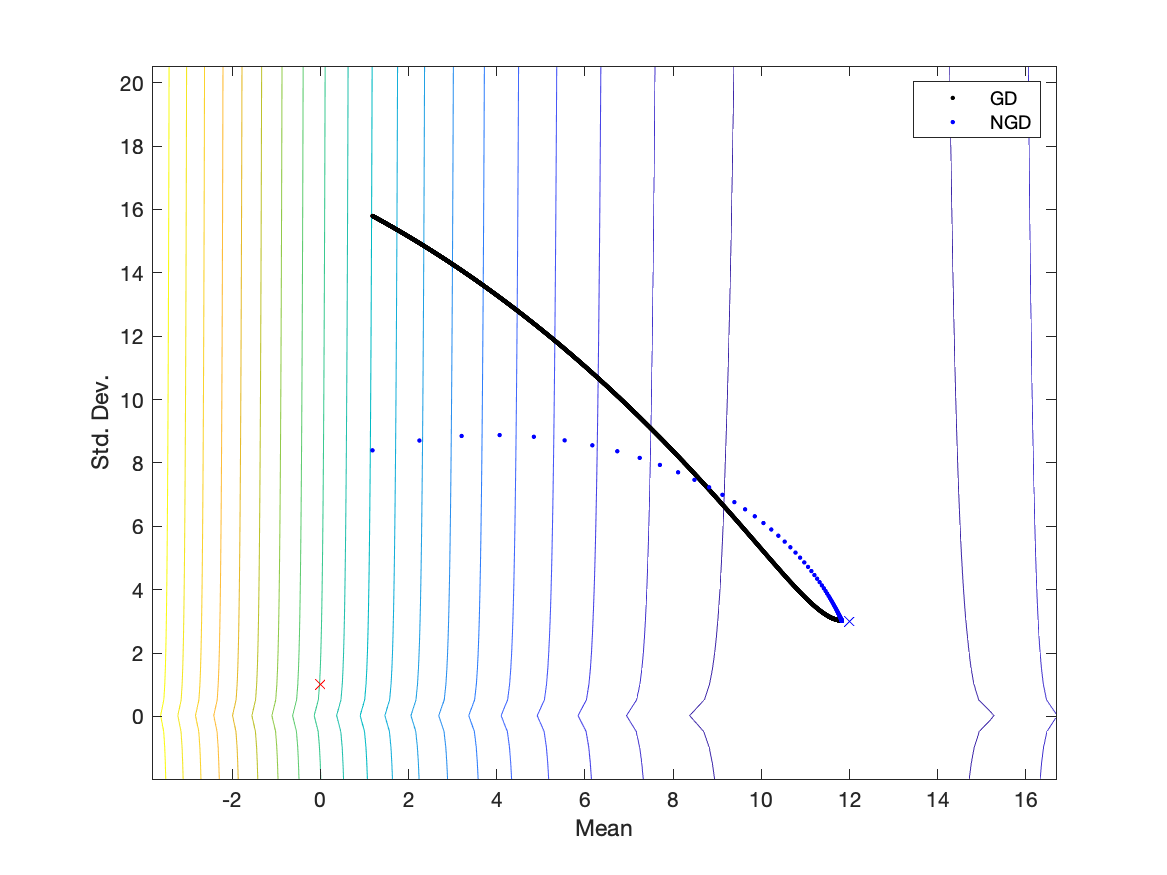
\includegraphics[scale=0.4]{img/MLE-iterations.png}
    \caption{Gradient descent and natural gradient descent finding the optimal parameters $\mu = 12, \sigma = 4$, starting with initial parameters $\mu = 0, \sigma = 1$. Both methods used a fixed step size of $1 \times 10^{-4}$.}
    \label{fig:MLE}
\end{figure}

In order to compare the two methods, the same fixed step size was used for both. From the resulting iterations, it can be seen that while gradient descent makes little progress per update (so that the individual points on the graph seem to form a continuous line) and is initially driven away from the global optimum, natural gradient descent is able to make considerable progress at every update and is not driven nearly as far away from the global optimum at the beginning.

Both methods exhibit a large parameter jump at the beginning of training, and this, along with the overall performance difference, can be explained by examining the gradients at each particular point on this space. The gradients and natural gradients are compared in figure \ref{fig:MLE-grads}.

\begin{figure}[H]
  \centering
  \subfloat{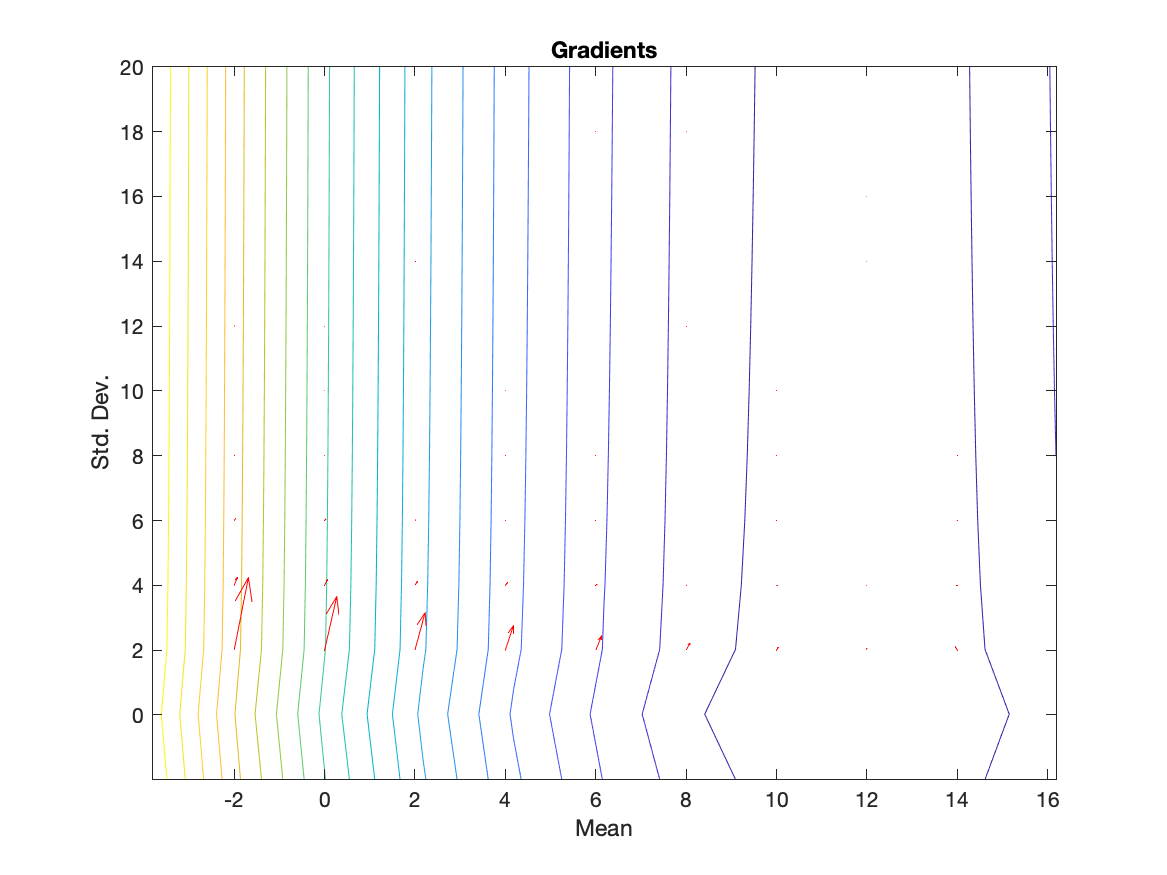
\includegraphics[width=0.45\textwidth]{img/normal-grad.png}}
  \subfloat{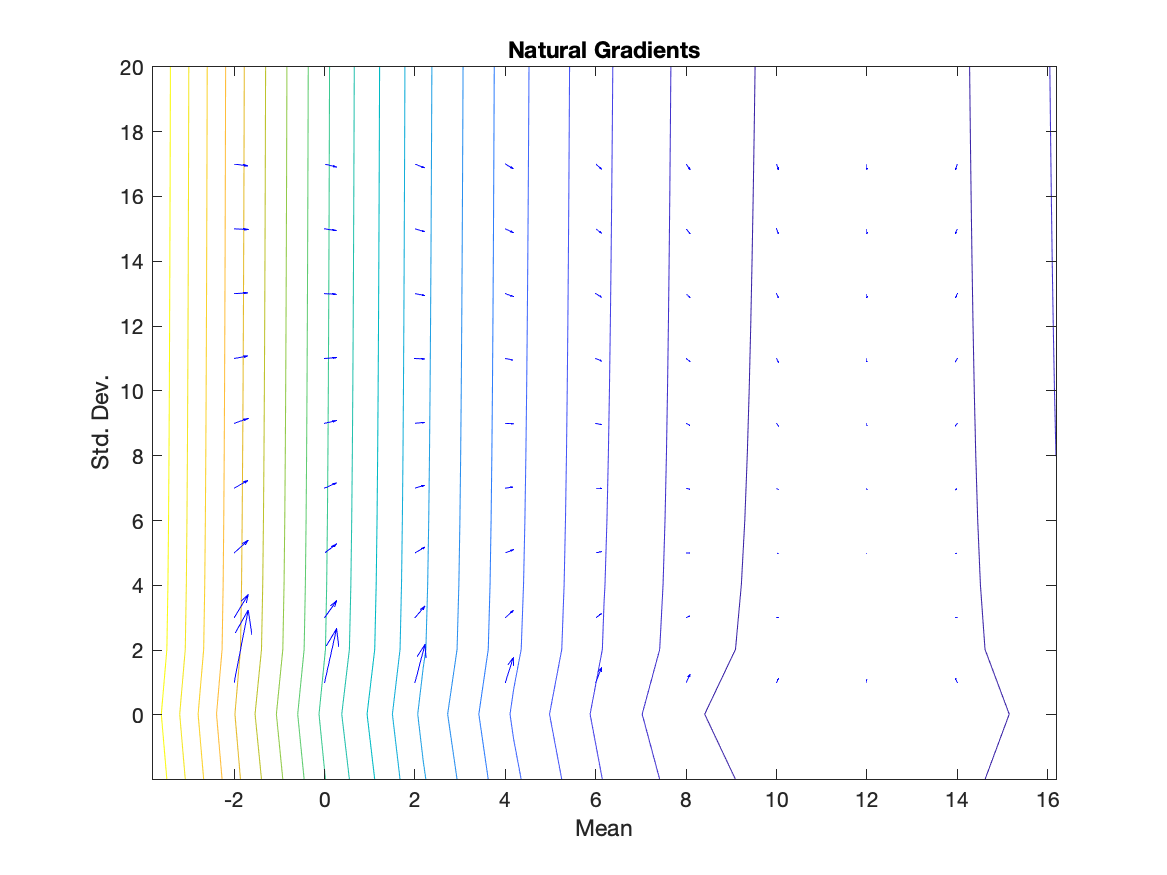
\includegraphics[width=0.45\textwidth]{img/natural-grad.png}}
  \caption{The gradients and natural gradients for the MLE problem. The natural gradients can be seen to be more similar in length, allowing for more normalized progress to be made in this space. The unmodified gradients, on the other hand, grow dramatically as the standard deviation approaches 0.}
  \label{fig:MLE-grads}
\end{figure}

From this figure it is clear that the initial parameter jump is due to the magnitude of the gradients growing as the mean approaches 0. In the case of gradient descent, however, these gradients grow unchecked, dwarfing the other gradients pictured. The small gradient magnitudes for larger values of $\mu$ explain why such little progress is made per iteration with the gradient descent scheme, and the initial large gradient magnitudes cause instability when the learning rate is increased.

The natural gradient, on the other hand, does not exhibit this behavior. Instead, its gradients are more comparable in magnitude, with the initial gradients not increasing $\mu$ as much and the later gradients pushing both parameters closer to the optimum as a faster rate.

This example demonstrates that we can solve optimization problems in probability space more effectively by using the natural gradient instead of just the gradient; however, this can be extended to cases beyond just supervised machine learning. One such application is policy improvement in reinforcement learning.

% ======================
% REINFORCEMENT LEARNING
% ======================
\subheader{Reinforcement Learning}

Given some agent acting in an arbitrary environment, reinforcement learning (RL) methods attempt to optimize the agent's performance using, in a rough sense, trial and error. We model the agent and environment as follows: let $\mathcal{S}$ denote the set of all possible states of the environment and $\mathcal{A}$ the set of all possible agent actions. Let $s_t$ denote the state of the environment at time $t$, and $a_t$ the action of the agent at time $t$. The environment is assumed to operate with Markovian transition dynamics, i.e., the next state of the environment depends only on the current state and action. We denote the transition dynamics with the distribution $p(s_{t+1} | s_t, a_t)$, although we will assume that this distribution is unknown. As the agent interacts with its environment, it generates a trajectory $\tau = (s_0, a_0, s_1, a_1, \dots, s_T)$, where $T$ is some terminal time step (which can be set to $\infty$ for tasks with no explicit end point).

The agent can be said to act according to some policy $\pi(a_t \vert s_t)$, where $\pi$ is a distribution of actions $a_t$ conditioned on the current state of the environment $s_t$. The policy $\pi$ need not be represented explicitly, although it is always at the very least induced by some action selection process. The agent's desired task is represented with a reward function $r: \mathcal{S} \times \mathcal{A} \to \mathbb{R}$, which takes in the state of the environment and the action performed by the agent and produces a real number that quantifies how well the agent is performing. The goal of RL can then be restated as trying to find the policy $\pi$ that maximizes evaluations of this reward function throughout the agent's interactions with the environment. This yields the classical RL objective
\begin{gather*}
    J(\pi) = \mathbb{E}_{\pi} \Big[ \sum_{t=0}^T r(s_t, a_t) \Big].
\end{gather*}
 The optimal policy is then $\pi^* = \arg\max_\pi J(\pi)$. One strategy for finding this optimal policy is to directly parameterize the policy with some $\theta$, which we can denote $\pi_\theta$. We define a new objective
\begin{gather*}
    \tilde{J}(\theta) = \mathbb{E}_{\pi_\theta} \Big[ \sum_{t=0}^T r(s_t, a_t) \Big],
\end{gather*}
which is just the original objective but written as a function of $\theta$ and using the parameterized version of the policy. A simple and reasonable method of maximizing this new objective is running gradient ascent on it with respect to $\theta$. Such methods are referred to as ``policy gradient" methods.


% =======================
% POLICY GRADIENT METHODS
% =======================
\subheader{Policy Gradient Methods and the Natural Gradient}

The most basic policy gradient method has the update scheme
\begin{gather*}
    \theta \gets \theta + \alpha \nabla_\theta \tilde{J}(\theta).
\end{gather*}
In this case, all we must calculate is the gradient term. During this calculation, it will be helpful to know the structure of the density of some trajectory $\tau$. We denote the density of $\tau$ conditioned on the current policy $p(\tau \vert \pi_\theta)$. Since the environment has Markovian dynamics, this density is
\begin{gather*}
    p(\tau \vert \pi_\theta) = \rho(s_0) \prod_{t=0}^T \pi_\theta(a_t | s_t) p(s_{t+1} | s_t, a_t),
\end{gather*}
where $\rho(s_0)$ denotes the initial state distribution of the environment. As it will be useful later, we can also calculate the logarithm of this expression
\begin{gather*}
    \log p(\tau \vert \pi_\theta) = \log \rho(s_0) + \sum_{t=0}^T \log \pi_\theta(a_t | s_t) + \log p(s_{t+1} | s_t, a_t).
\end{gather*}
We now begin calculating the gradient term in the gradient ascent scheme.
\begin{align*}
    \nabla_\theta \tilde{J}(\theta) &= \nabla_\theta \mathbb{E}_{\pi_\theta} \Big[ \sum_{t=0}^T r(s_t, a_t) \Big] \\
    &= \nabla_\theta \int p(\tau \vert \pi_\theta) \sum_{t=0}^T r(s_t, a_t) \,d\tau \\
    &= \int \nabla_\theta p(\tau \vert \pi_\theta) \sum_{t=0}^T r(s_t, a_t) \,d\tau.
    \intertext{By examining the expression for $\nabla_\theta p(\tau \vert \pi_\theta)$ above, it is clear that the gradient will rely on the transition dynamics. Since the dynamics are unknown, we cannot calculate this. We can, however, use the identity $\nabla \log x = \frac{\nabla x}{x}$ to transform the integral.\cite{pg}}
    &= \int p(\tau \vert \pi_\theta) \nabla_\theta \log p(\tau \vert \pi_\theta) \sum_{t=0}^T r(s_t, a_t) \,d\tau \\
    &= \mathbb{E}_{\pi_\theta} \Big[ \nabla_\theta \log p(\tau \vert \pi_\theta) \sum_{t=0}^T r(s_t, a_t) \Big].
    \intertext{By examining the expression for the log density of $\tau$, we see that the gradient of this term does \textit{not} rely on the transition dynamics and instead relies only on $\log \pi_\theta$. Our final gradient expression is}
    \nabla_\theta \tilde{J}(\theta) &= \mathbb{E}_{\pi_\theta} \bigg[ \bigg( \sum_{t=0}^T \nabla_\theta \log \pi_\theta(a_t \vert s_t) \bigg) \bigg( \sum_{t=0}^T r(s_t, a_t) \bigg) \bigg].
\end{align*}
Since we control $\theta$, we can determine the form of $\pi_\theta$ and know how to calculate log densities. Thus we can calculate the terms inside the expectation exactly, and the expectation itself we can approximate using sampling\cite{pg}.

This allows us to define a more explicit policy gradient algorithm in which we sample multiple trajectories, calculate the above expectation using these samples, and then use this to perform a gradient update on the parameters of our policy.

{\centering
\begin{minipage}{0.7\linewidth}
\begin{algorithm}[H]
    \caption{Basic Policy Gradient}
    \label{alg:PG}
    \begin{algorithmic}
        \Require $N$, step size $\alpha$, initial $\theta$
        \While{not converged}
            \State Sample $\{ \tau_i \}_{i=1}^N$
            \State $g \gets \frac{1}{N} \sum_{i=1}^N \big( \sum_{t=0}^T \nabla_\theta \log \pi_\theta(a_t \vert s_t) \big) \big( \sum_{t=0}^T r(s_t, a_t) \big)$
            \State $\theta \gets \theta + \alpha g$
        \EndWhile
    \end{algorithmic}
\end{algorithm}
\end{minipage}
\par}
\vspace{7mm}

One shortcoming of this algorithm is its data inefficiency. Multiple trajectories are needed to gain an accurate estimation of the policy gradient, but gaining multiple trajectories requires many interactions with the environment.

To address this inefficiency, we can take natural gradient steps instead.\cite{npg} We saw that the natural gradient made maximum likelihood estimation more efficient, so it is reasonable to assume that it may have a similar effect here. Since the policy gradient method operates in probability space, using the natural gradient is equivalent to left multiplying the policy gradient by the inverse of the Fisher information matrix. This gives us the natural policy gradient method, which uses the same sampling approximations as in Algorithm~\ref{alg:PG}.

{\centering
\begin{minipage}{0.7\linewidth}
\begin{algorithm}[H]
    \caption{Natural Policy Gradient}
    \label{alg:NPG}
    \begin{algorithmic}
        \Require $N$, step size $\alpha$, initial $\theta$
        \While{not converged}
            \State Sample $\{ \tau_i \}_{i=1}^N$
            \State $F \gets \frac{1}{T N} \sum_{i=1}^N \sum_{t=0}^T \big( \nabla_\theta \log \pi_\theta(a_t \vert s_t) \big) \big( \nabla_\theta \log \pi_\theta(a_t \vert s_t) \big)^T$
            \State $g \gets \frac{1}{N} \sum_{i=1}^N \big( \sum_{t=0}^T \nabla_\theta \log \pi_\theta(a_t \vert s_t) \big) \big( \sum_{t=0}^T r(s_t, a_t) \big)$
            \State $\theta \gets \theta + \alpha F^{-1} g$
        \EndWhile
    \end{algorithmic}
\end{algorithm}
\end{minipage}
\par}
\vspace{7mm}

To compare the natural policy gradient with the policy gradient, we can construct a toy environment with a simple task. Let the state space simply be the real number line, and let the agent start at the origin. At every time step, it samples a number from a Gaussian $\mathcal{N}(\mu, \sigma^2)$ and moves that distance from its current location. If we want the agent to simply learn to do nothing, then we can define the reward function to be $r(s,a) = -s^2 - a^2$. The performance of both algorithms in learning the optimal $\mu$ and $\sigma$ in this environment are shown in Figure~\ref{fig:PG}.

\begin{figure}[H]
    \centering
    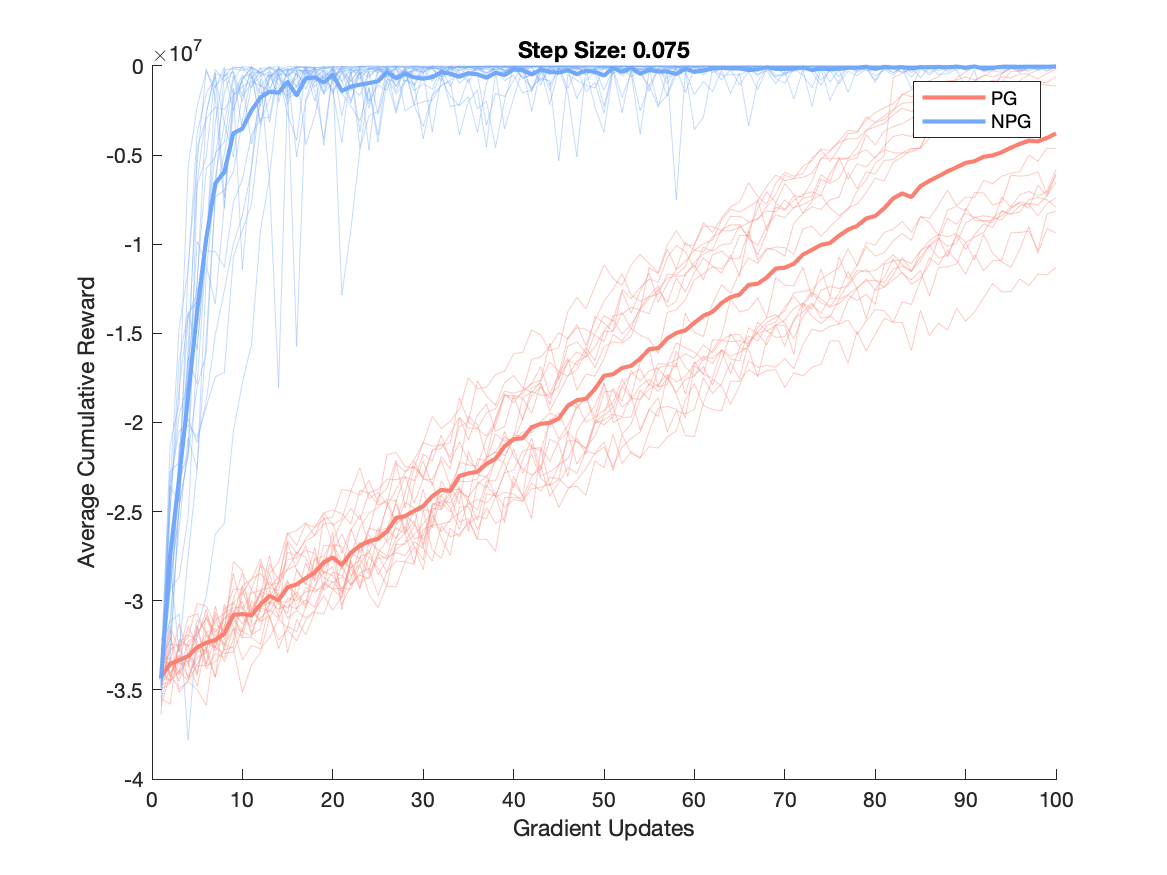
\includegraphics[scale=0.4]{img/PG-reward.png}
    \caption{The average cumulative reward of ten agents trained by the policy gradient (PG) and natural policy gradient (NPG) on the toy environment, with the average reward across all ten agents denoted by the bold lines. Both methods used the fixed step size 0.075.}
    \label{fig:PG}
\end{figure}

Beginning with poorly-chosen initial parameters $\mu = 10$ and $\sigma = 14$, the natural policy gradient was able to quickly minimize $\mu$ and $\sigma$, compared to the basic policy gradient. Calculating the explicit natural gradients for this scenario shows that the terms of the natural gradient are just those of the gradient but multiplied by $\sigma^2$ and an additional constant. This allows for larger steps at the beginning of training when $\sigma$ is large. This combats a particular problem posed by this toy environment, which is that the gradient term corresponding to $\sigma$ is low compared to the gradient term corresponding to $\mu$. This causes the variance of the policy to remain high for many iterations, which leads to many sub-optimal actions and the slow learning of the policy gradient.\cite{peters-schaal}

This particular environment allowed for a simple policy with few parameters, but for more general policies, many parameters are necessary. In this case, the Fisher information matrix is expensive to construct and invert. An efficient calculation of the Fisher information matrix must then be developed.

\subheader{Efficiently Calculating the Fisher Information Matrix}

Instead of forming and then inverting the Fisher information matrix, it is of computational benefit to instead calculate just the matrix vector product $g = F^{-1} \nabla_\theta J(\theta)$. If we left-multiply both sides of this equation by $F$, we get $F g = \nabla_\theta J(\theta)$. Then if we have access to a function that maps $g \to F g$, we can solve this system of equations without ever explicitly forming $F$ or $F^{-1}$. One possible choice for solving this system is using the conjugate gradient method, which was employed successfully in the Trust Region Policy Optimization algorithm, a modification of the natural policy gradient with performance improvement guarantees.\cite{trpo}

\subheader{Conclusion}

We saw that the natural gradient extends gradient descent into general metric spaces, which is especially useful when optimizing probabilistic models. We also saw that the natural gradient can increase the efficiency of reinforcement learning algorithms. In fact, it plays a major role in most state-of-the-art reinforcement learning methods. For example, the aforementioned Trust Region Policy Optimization is a recent extension of the natural gradient,\cite{trpo} and Proximal Policy Optimization uses the connection between the natural gradient and KL divergence to relax the trust region constraint for more efficient policy updates.\cite{ppo}

It is also possible to derive completely different optimization methods using the same trust region formulation. It is possible to limit policy updates using the Wasserstein distance from optimal transport theory instead of KL divergence.\cite{wgf} Such methods can be shown to have ties to the natural gradient that we derived.\cite{ng-ot} This also shows potential connections between reinforcement learning and generative modeling, the latter of which commonly uses Wasserstein distances. The extent of the connections between these two branches of machine learning and the effect of trust regions on optimizing generative models are outside the scope of this paper, but are potential areas for future research.

% \newpage
%\subheader{References}

\begin{thebibliography}{0}

\bibitem{amari} Amari, S., 1997. Neural Learning in Structured Parameter Spaces - Natural Riemannian Gradient, in: Mozer, M.C., Jordan, M.I., Petsche, T. (Eds.), Advances in Neural Information Processing Systems 9. MIT Press, pp. 127–133.

\bibitem{deep-linear-ng} Bernacchia, A., Lengyel, M., Hennequin, G., 2018. Exact natural gradient in deep linear networks and its application to the nonlinear case, in: Bengio, S., Wallach, H., Larochelle, H., Grauman, K., Cesa-Bianchi, N., Garnett, R. (Eds.), Advances in Neural Information Processing Systems 31. Curran Associates, Inc., pp. 5941–5950.

\bibitem{npg} Kakade, S.M., 2002. A Natural Policy Gradient, in: Dietterich, T.G., Becker, S., Ghahramani, Z. (Eds.), Advances in Neural Information Processing Systems 14. MIT Press, pp. 1531–1538.

\bibitem{empirical-fim} Kunstner, F., Balles, L., Hennig, P., 2019. Limitations of the Empirical Fisher Approximation for Natural Gradient Descent. arXiv:1905.12558 [cs, stat].

\bibitem{ng-ot} Li, W., Montufar, G., 2019. Natural gradient via optimal transport. arXiv:1803.07033 [cs, math].

\bibitem{deep-ng} Pascanu, R., Bengio, Y., 2014. Revisiting Natural Gradient for Deep Networks. arXiv:1301.3584 [cs].

\bibitem{peters-schaal} Peters, J., Schaal, S., 2008. Reinforcement learning of motor skills with policy gradients. Neural Networks, Robotics and Neuroscience 21, 682–697.

\bibitem{ng-deriv} Ratliff, N., n.d. Information Geometry and Natural Gradients 8.

\bibitem{trpo} Schulman, J., Levine, S., Moritz, P., Jordan, M.I., Abbeel, P., 2017a. Trust Region Policy Optimization. arXiv:1502.05477 [cs].

\bibitem{ppo} Schulman, J., Wolski, F., Dhariwal, P., Radford, A., Klimov, O., 2017b. Proximal Policy Optimization Algorithms.

\bibitem{pg} Sutton, R.S., McAllester, D.A., Singh, S.P., Mansour, Y., 2000. Policy Gradient Methods for Reinforcement Learning with Function Approximation, in: Solla, S.A., Leen, T.K., Müller, K. (Eds.), Advances in Neural Information Processing Systems 12. MIT Press, pp. 1057–1063.

\bibitem{tr} Yuan, Y., 1999. A Review of Trust Region Algorithms for Optimization. ICM99: Proceedings of the Fourth International Congress on Industrial and Applied Mathematics.

\bibitem{wgf} Zhang, R., Chen, C., Li, C., Carin, L., 2018. Policy Optimization as Wasserstein Gradient Flows.

\end{thebibliography}
\newpage



\appendix

\section{Alternate Form of the Fisher Information Matrix}
\label{appendix:FIM}
The matrix $F = -\int p_{\theta_t}(x) \nabla^2 \log p_{\theta_t}(x) \,dx$ is in fact the Fisher Information matrix, as shown below. All gradients in the following derivation are implicitly taken with respect to $\theta_t$. We begin by expanding $\nabla^2 \log p_{\theta_t}(x)$.

\begin{align*}
    \nabla^2 \log p_{\theta_t}(x) &= \nabla \frac{\nabla p_{\theta_t}(x)}{p_{\theta_t}} \\
    &= \frac{p_{\theta_t}(x) \nabla^2 p_{\theta_t}(x) - \nabla p_{\theta_t}(x) \nabla p_{\theta_t}(x)^T}{p_{\theta_t}(x)^2} \\
    &= \frac{\nabla^2 p_{\theta_t}(x)}{p_{\theta_t}(x)} - \frac{\nabla p_{\theta_t}(x) \nabla p_{\theta_t}(x)^T}{p_{\theta_t}(x)^2}
    \intertext{Using the identity $\nabla \log x = \frac{\nabla x}{x}$, we can simplify the rightmost fraction.}
    &= \frac{\nabla^2 p_{\theta_t}(x)}{p_{\theta_t}(x)} - \nabla \log p_{\theta_t}(x) \nabla \log p_{\theta_t}(x)^T
\end{align*}
Plugging this into the definition of $F$ yields
\begin{align*}
    F &= -\int p_{\theta_t}(x) \nabla^2 \log p_{\theta_t}(x) \,dx \\
    &= \int p_{\theta_t}(x) \nabla \log p_{\theta_t}(x) \nabla \log p_{\theta_t}(x)^T \,dx - \int \nabla^2 p_{\theta_t}(x) \,dx \\
    &= \mathbb{E}_{x \sim p_{\theta_t}} \big[ \nabla \log p_{\theta_t}(x) \nabla \log p_{\theta_t}(x)^T \big] - \nabla^2 \int p_{\theta_t}(x) \,dx \\
    &= \mathbb{E}_{x \sim p_{\theta_t}} \big[ \nabla \log p_{\theta_t}(x) \nabla \log p_{\theta_t}(x)^T \big] - \nabla^2 \mathbf{1} \\
    &= \mathbb{E}_{x \sim p_{\theta_t}} \big[ \nabla \log p_{\theta_t}(x) \nabla \log p_{\theta_t}(x)^T \big]
\end{align*}
which is the definition of the Fisher information matrix.

\end{document}
